\section{Busqueda de un dataset}
\label{sec:busquedaDataset}
Para poder entrenar modelos de \gls{ia} se requiere una gran cantidad de datos, en este caso de animaciones de los gestos escogidos que se han mencionado en la introducción.
Además, estos datos tienen que estar en un formato en el que se pueda extraer la información de los huesos (posición y rotación) para que pueda ser usado por los modelos, y tenían que ser compatibles con los huesos del traje de captura de movimiento.

\subsection{Dataset de la Universidad Carnegie Mellon}
La Universidad privada Carnegie Mellon, ubicada en Pittsburgh, Pensilvania, tiene dispoible de forma gratuita un dataset de movimientos recogidos mediante la captura de movimiento.\footnote{Enlace a la página del dataset de la Universidad Carnegie Mellon: \url{https://mocap.cs.cmu.edu/}}
Sin embargo este dataset no ha sido posible utilizarlo por tres motivos.

El primer motivo es la incompatibilidad del esqueleto utilizado por ellos con el utilizado por el traje de captura de movimiento Perception Neuron 3.
Como se puede ver en \cite{MCUINFO} su traje contiene 41 puntos usados para la captura, mostrados en la figura \ref{fig:MCUTraje}, dando a lugar al esqueleto mostrado en la misma figura.

\begin{figure}[H]
	\centering
	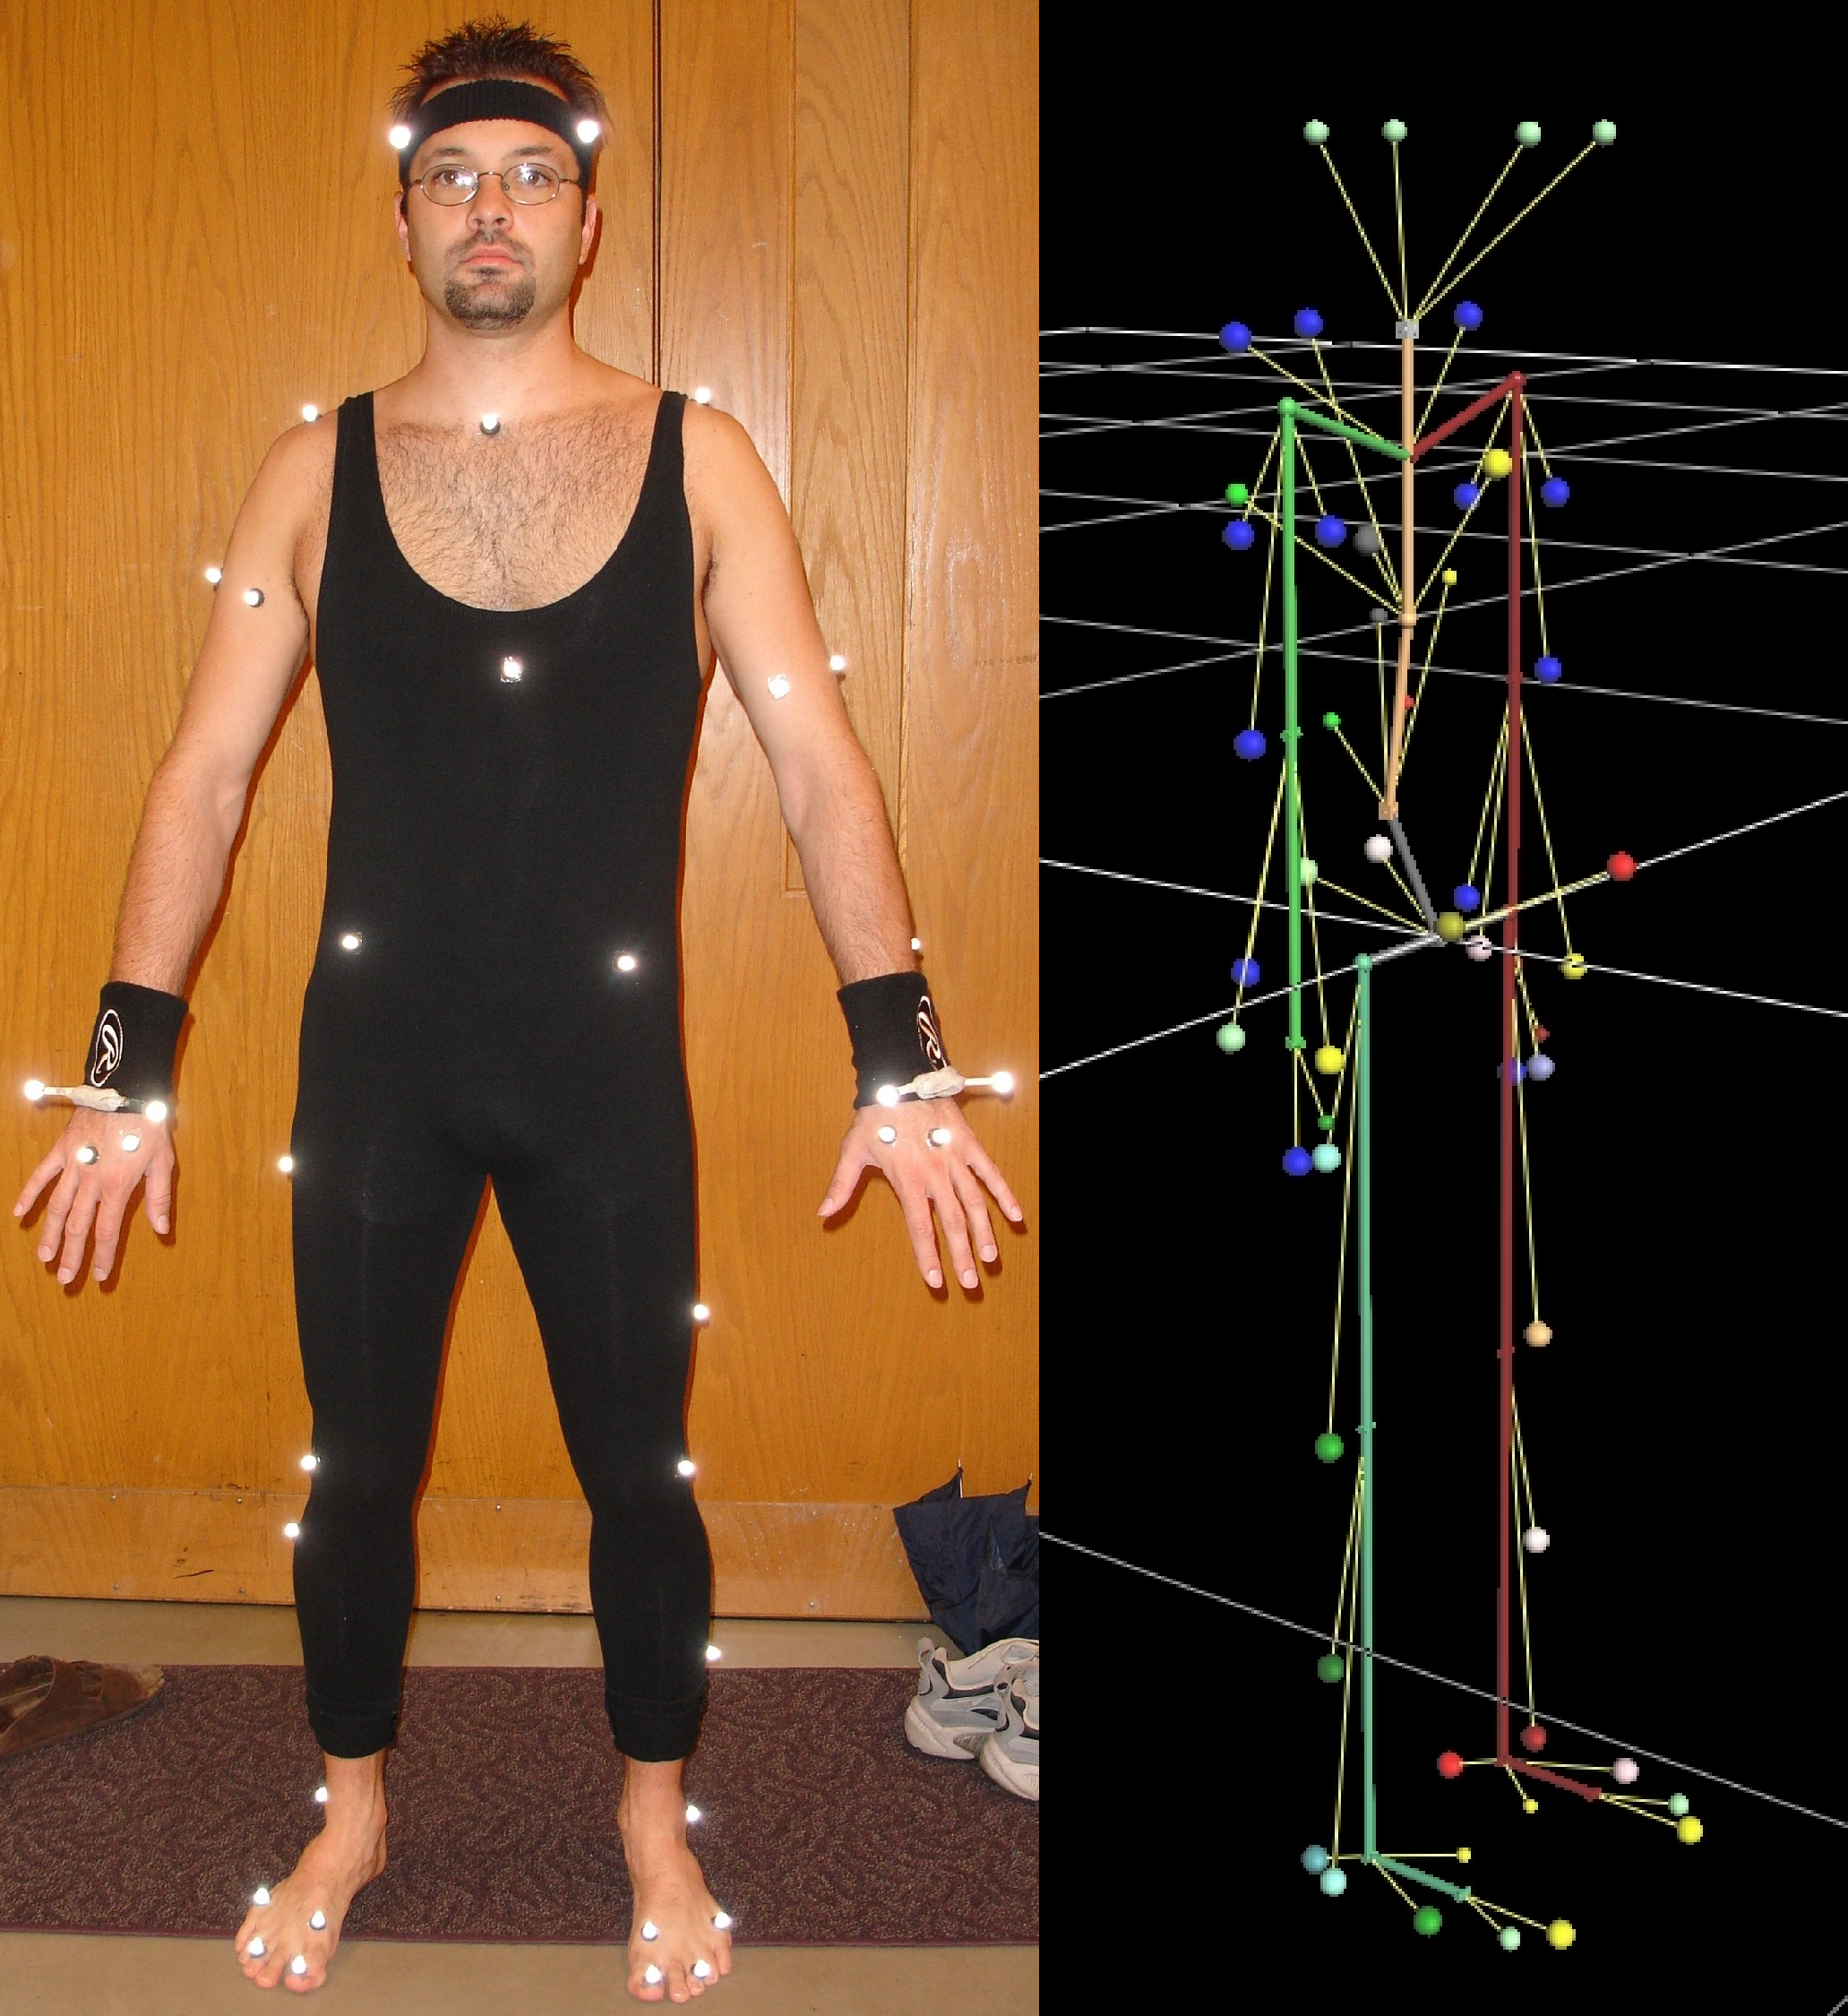
\includegraphics[width=0.5\textwidth]{Imagenes/Vectorial/TrajeMCU.pdf}
	\caption{Imágen del traje de captura de movimiento utilizado para la base de datos de la Universidad Carnegie Mellon (izquierda) y el esqueleto resultante (derecha). Fuente: \url{https://mocap.cs.cmu.edu/info.php}}
	\label{fig:MCUTraje}
\end{figure}


Por otro lado, como ya mencionamos en el capítulo \ref{sec:traje}, el traje Perception Neuron 3 contiene 17 puntos, por lo que debido a las grandes diferencias de los esqueletos decidimos no utilizarlos.

El segundo motivo por el que no se ha usado el dataset de la Universidad Carnegie Mellon es el formato de las animaciones disponibles.
Las animaciones presentes en el dataset vienen en tres formatos distintos: c3d, asf (o amc) y vsk (o v).
Los formatos c3d, vsk y v son unos formatos en binario usados para objetos en 3D, por lo que no se puede usar de forma sencilla para extraer la información del propio archivo.
Por otro lado los archivos asf y amc son archivos en formato ASCII con la información de los huesos. Sin embargo la documentación aportada para poder usar la información es incompleta.

El último motivo por el que no se ha usado este dataset es por la escasez de animaciones de los gestos buscados.
Animaciones como ``correr'' sí están presentes (aunque no en abundancia), pero otras como ``pelear'' o ``saludar'' no.

Este último problema también ha estado presente en páginas específicas de bancos de datasets como Kaggle.

\subsection{Kaggle}

Kaggle es una página web dedicada a la ciencia de datos y el aprendizaje automático y la \gls{ia}. En Kaggle se pueden encontrar datasets, modelos, código y competiciones de \gls{ia}. Kaggle tiene una gran comunidad de usuarios y una gran selección de datasets para distintas finalidades.

En un primer momento, se pensó en usar datasets de imágenes/vídeo, así que se buscó conjuntos de datos de este formato. La búsqueda no obtuvo los resultados esperados, ya que no se encontró datos de poses generales como las requeridas, y en concreto no se consiguió mucha cantidad de datos.

Tras analizar las desventajas de usar imágenes y videos, se pensó que era mejor usar un conjunto de datos basado en animaciones (o coordenadas de las mismas). Algunas de estas desventajas consideradas fueron:
\begin{itemize}
    \item Complejidad de renderizado: las imagenes y/o vídeos requerirían de renderizar una cámara externa dentro del motor para capturar la presencia del usuario. Esto ya requeriría más potencia de computo, sin contar lo que requeriría el modelo.
    \item Transferencias de datos más grandes: al plantear un servidor para el modelo, se pensó en el tamaño de las imágenes que habría que mandar para hacer las inferencias. En el caso de tener una red de velocidad limitada sería mejor mandar los puntos concretos del traje que mandar imágenes completas. Las imágenes, incluso al ser de baja calidad, requerirían una cantidad muy grande de píxeles para hacer el modelo del usuario fácilmente reconocible.
    \item Perdida de contexto: el traje de captura de movimiento te permite obtener datos tridimensionales de cada punto por defecto, sin necesidad de tener que recrear un esqueleto 3D con capas extra en el modelo.
\end{itemize}

Tras este cambio de enfoque, se buscó datasets de animaciones y modelos 3D. Resultó ser una búsqueda incluso peor que la anterior, ya que por la limitación de gente que tiene acceso a trajes de captura de movimiento, no había datasets públicos en dataset con este tipo de datos.

Ya que no se encontró un gran dataset que cumpliese con nuestros requerimientos se tomó la decisión de buscar en un banco de animaciones los gestos requeridos y transformar esas animaciones en un formato que puediesen ser procesados.